\chapter{Alternative to SA: Highly Parallel Nonequilibrium Switching}

\section{Introduction}
%
As discussed, there are several limitations of the stochastic approximation (SA) algorithm.
%
However, that does not preclude the use of the reversible-jump (RJ) algorithm in other clever ways.
%
For a long time, it has been known that rather than accepting or rejecting a proposal attempt, one can cache the resulting acceptance probability and use it to estimate the free energy difference offline.
%
In molecular simulation, this technique is known as nonequilibrium switching~\cite{Hummer2001, Aldeghi2018}, and in statistics as annealed importance sampling (AIS)~\cite{Neal2001}.
%
Examples of estimation techniques include the exponential averaging estimator~\cite{Zwanzig1954}, as well as the optimal Bennett Acceptance Ratio (BAR)~\cite{Bennett1976,Shirts2005,Crooks1999Thesis, Meng1996}, which uses bidirectional data.
%
Though this has not often been utilized for free energy calculations, it has several appealing advantages in the modern age.
%
First, it is highly parallelizable--unlike SAMS-like expanded ensemble algorithm, it can easily run many switching trajectories or proposal attempts simultaneously.
%
With hardware becoming increasingly parallel and the availability of cloud computing, this is an attractive feature.
%
Second, there is no need to wait for a sampler to explore all the states--by definition of the algorithm, the user can choose which states.
%
Third, it is still possible to employ a wide range of adaptive algorithms.
%
For instance, one could use Bayesian experimental design~\cite{Vanlier2012, DasGupta1996} to iteratively choose how to allocate effort to different "legs" of the calculation.
%
\section{Advantage of RJ Nonequilibrium Switching}
%
Since codes for nonequilibrium switching based relative free energy calculations already exist, one might wonder what advantage the complication of reversible jump brings.
%
In order to understand why one would undertake this approach, consider what is required for a standard nonequilibrium switching based relative free energy calculation.
%
In Figure~\ref{fig:trad_neq}, one can see that the typical setup of a nonequilibrium free energy calculation is to run simulations at the alchemical endpoints (that is, a hybrid system with the control parameters set to either 1.0 or 0.0), and periodically generate proposal attempts to reach the other endpoint.
%
This requires simulation of the hybrid system at both endpoints for each pair for which one would like to calculate the free energy difference.
%
Note that in this scheme, one cannot use the equilibrium simulation used in a calculation for $\Delta\Delta_{AB}$ to, for instance, estimate $\Delta\Delta_{AC}$, where $A,B,C$ are molecule indices.
%
This is because the alchemical system must contain all the degrees of freedom of both endpoints, which will not necessarily include the degrees of freedom of the rest.
%
\begin{figure}
    \centering
    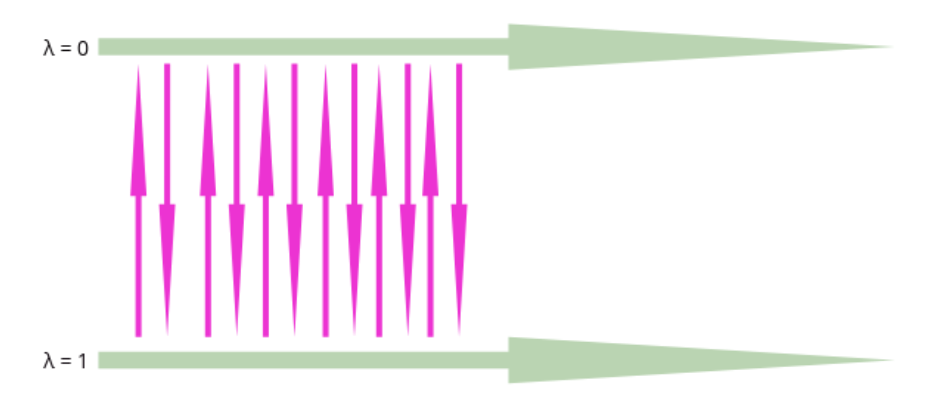
\includegraphics[width=1.0\textwidth]{new_neqdiagram.png}
    \caption{Illustration of a nonequilibrium switching free energy calculation. Note the requirement for simulation at the alchemical endpoints. The horizontal green lines represent the equilibrium simulations at each endpoint, while the magenta lines depict the switching trajectories from samples of each state to the other.}
    \label{fig:trad_neq}
\end{figure}
%
However, using the reversible jump scheme, one simulates from the \emph{nonalchemical} endpoints for each molecule, and then in the course of the nonequilibrium switching trajectory, inserts the missing degrees of freedom and removes the superfluous degrees of freedom.
%
This means that, to use the previous abstract example, one can simply run multiple equilibrium simulations, then adaptively choose which pairs should be emphasized.
%
It would also allow new molecules to be added without re-simulating any of the existing molecules in the set; in principle, if one wanted a fast estimate, the exponential averaging estimator could even be used to without performing any additional equilibrium simulation.
%
Additionally, the reversible jump scheme enables ring formation and breakage without resorting to more sophisticated tricks, which allows a much greater freedom for the user to choose different 
%
Finally, an adaptive design scheme based on Bayesian experimental design could easily incorporate other non-free-energy-based objectives, such as a model of synthetic accessibility or some other desirability criterion.
%
\section{Use of cloud computing resources}
%
This approach to the reversible-jump based algorithm presented in this thesis opens the door to ready use of cloud resources such as Amazon Web Services, which are already being employed in free energy simulations~\cite{Cournia2017}.
%
Offerings such as AWS not only enable users without in-house clusters to use high-performance hardware, but also enhance the reproducibility of research.
%
Entire stacks used to perform computation can be exported via services such as AWS CloudFormation, enabling rapid and straightforward reproduction of research.
%
Another benefit of using on-demand cloud resources is that it enables the direct application of economics to the question of calculation efficiency.
%
Rather than comparing algorithms in terms of asymptotic variance or other similar criteria, we can now compare them in terms of their dollar cost; how much do we have to spend in order to achieve the desirable result?
%
This also allows us to put a direct price tag on speed improvements.
%
While questions such as the variance of the acceptance probability once seemed abstract, they now strike our wallets.
%
Since we are performing calculations on groups of molecules, we can also use this cost data to determine which edges are most profitable to explore, and which can be estimated by summing other edges.
%
As in \cite{Wang2015}, the presence of cycles could also be used to correct for errors in the calculation.
%
\section{Pricing and Economics of Cloud Computing}
%
Due to familiarity, the remainder of this chapter will use Amazon Web Services as an example.
%
Using AWS for molecular simulation, there are several cost considerations:
\begin{itemize}
    \item Storage of input and output
    \item Compute time
    \item Data egress (ingress is free)
\end{itemize}
%
Here, I will primarily discuss the issue of compute time.
%
There are several pricing models on AWS and its competitors for compute time.
%
On-demand pricing refers to the use of resource at a fixed hourly price.
%
So-called spot pricing allows users to bid on unused capacity at a significantly reduced price.
%
This price fluctuates, however, and is not guaranteed to remain under the user's bid.
%
In the present situation, this is tolerable: if an instance is killed because it becomes prohibitively expensive, we lose whatever nonequilibrium switching it has performed but not copied to storage, but nothing else.
%
At the time of this writing and in the geographically nearest datacenter, the price of a single GPU instance hovered near \$0.27 per hour.
%
In preliminary investigations on a GTX-Titan, a full proposal of 10ps from one alkane to another takes approximately 60 seconds.
%
In other words, we can compute over 100 switching attempts for just 50 cents!
%
Of course, this is a small system--scaling up will be pricier. 
%
These price signals can also guide the investigator into the most effective use of his or her time and money.
%
However, this illustrates the low cost of the algorithm on modern infrastructure, and also highlights that pairs of molecules for which is advantageous to compute many switching attempts can be done cheaply and in parallel.
%
One may be left wondering why one couldn't simply use many replicates of the stochastic approximation algorithm to take advantage of the parallelism.
%
One could do this, of course, and whether this is efficient in terms of processor or wall clock time requires empirical investigation.
%
However, one feature of the low spot pricing is its volatility--a user cannot rely on the price remaining at its current level indefinitely.
%
In fact, this aspect has motivated interesting research in modeling the price of spot resources~\cite{Javadi2011} that can be brought to bear on this application.
%
Since the nonequilibrium switching trajectories are independent of each other, loss of some compute resources is not devastating.
%
If necessary, the number of nonequilibrium switching trajectories being performed in parallel can be reduced to save money when the cost increases.
%
Effort can be adaptively reallocated by whatever model or heuristic the user desires.
%
However, if one suspends a chain exploring chemical space due to cost, one loses the adaptation that that chain has already performed.
%
There may exist powerful methods of coupling the stochastic approximation weights, but this is a topic for future research.
%
\subsection{Factors affecting performance}
%
One factor affecting performance is the nonequilibrium protocol itself. 
%
Another factor that could potentially affect performance of this algorithm is the correlation time of the equilibrium simulation.
%
Unlike the SAMS case, where the algorithm accepts or rejects moves to different chemical states, this approach does not benefit from the potential decorrelating effect of changing chemical states.
%
Additionally, the number of parallel computing devices available will profoundly affect whether this choice is a feasible one.
%
With a large number of processing devices, this approach can reduce wall clock time, but empirical evaluation is necessary to determine whether for relative free energy calculations this approach is comparable in efficiency to equilibrium staging.